% Copyright 2002-2024 The University of Maryland Baltimore County (UMBC)
% 1000 Hilltop Circle, Baltimore, Maryland, 21250, USA
% https://www.csee.umbc.edu/

\documentclass[letter,10pt]{article}
\usepackage[breaklinks,pdfa=true,bookmarks=true,pdfdisplaydoctitle=true]{hyperref}
\hypersetup{
    unicode=false,          % non-Latin characters in Acrobat’s bookmarks
    pdftoolbar=true,        % show Acrobat’s toolbar?
    pdfmenubar=true,        % show Acrobat’s menu?
    pdffitwindow=false,     % window fit to page when opened
    pdfstartview={XYZ null null 1.00},    % disable zoom
    pdftitle={Problem Solving and Computer Programming Syllabus},    % title
    pdfauthor={Richard Zak},     % author
    pdfsubject={UMBC CMSC104 Problem Solving and Computer Programming},   % subject of the document
    pdfkeywords={Computer Science, Programming, Problem Solving, CSEE}, % list of keywords
    pdfnewwindow=true,      % links in new PDF window
    colorlinks=true,       % false: boxed links; true: colored links
    linkcolor=red,          % color of internal links (change box color with linkbordercolor)
    citecolor=green,        % color of links to bibliography
    filecolor=magenta,      % color of file links
    urlcolor=cyan           % color of external links
}
\usepackage{graphicx}
\usepackage{fancyhdr}
\pagestyle{fancy}
\usepackage[letterpaper, margin=1in]{geometry}
\geometry{letterpaper}
\usepackage{parskip} % Disable initial indent
\usepackage{color,soul} % Highligher
\usepackage[normalem]{ulem} % Strikethrough with \sout{}

\definecolor{cadmiumgreen}{rgb}{0.0, 0.42, 0.24}

\renewcommand{\today}{\number \day \ \ifcase \month \or January\or February\or March\or %
April\or May \or June\or July\or August\or September\or October\or November\or %
December\fi \ \number \year} 

\usepackage[utf8]{inputenc}
\fancyhf{}
\renewcommand{\headrulewidth}{0pt} % Remove default underline from header package
% \rhead{CMSC 104 Section 01: Problem Solving and Computer Programming}
% \lhead{\begin{picture}(0,0) \put(-65,-8){
\includegraphics[width=1.1cm]{Images/UMBC-vertical}} \end{picture}}
\fancyhead[L]{
    \makebox[\textwidth][s]{
        \begin{picture}(0,15){
\includegraphics[height=0.375in]{Images/UMBC-primary-logo-RGB.png}}
        \end{picture}
        \hspace{1.5cm} % Adjust space between image and text as needed
        CMSC 104 Section 01:\\\\Problem Solving and Computer Programming
    }
}
\cfoot{\thepage}
\rfoot{Fall 2024
}
\lfoot{CMSC 104 Section 01}
%\AtEndDocument{\vfill \LaTeX \hfill}
\AtEndDocument{\hfill \vfill Last modified: \today}

\begin{document}

\textbf{Semester:} Fall 2024
\\
\textbf{Location:} Engineering 122A \\
\textbf{Time:} Mondays \& Wednesdays 5:30 -- 6:45 \\
\textbf{Instructor:} Richard Zak \\
\textbf{Email:} \href{mailto:richard.zak@umbc.edu?Subject=CMSC104}{richard.zak@umbc.edu} \\
\textbf{Teaching Fellow:} Marcus Davis \\
\textbf{Email:} \href{mailto:marcusd2@umbc.edu?Subject=CMSC104}{marcusd2@umbc.edu}

\section*{Day/Hours Available}
\begin{itemize}
\item Approximately 30 minutes prior to class, if planned ahead.
\item At least 30 minutes after class, possibly longer.
\item Virtual meeting Tu/Th by appointment. Schedule via email, or at \url{https://calendly.com/rjzak/meeting}.
\item In Email: Anytime, and I will respond within 48 hours.
\end{itemize}

\section*{Course Description}
\paragraph{}This course is designed to provide an introduction to problem solving and computer programming that does not require prior programming experience. Elementary problem solving skills and algorithm development will be introduced. Students will be taught the basic use of a programming environment and basic programming constructs (including loops, control statements, functions, and arrays).

\paragraph{Note:}This course does not fulfill any of the computer science major requirements. Students who have taken and received transfer credit for, or who are taking concurrently any computer programming course in a high-level programming language, will not receive credit for CMSC 104. The list of such computer programming courses includes, but is not limited to AP Computer Science, CMSC 201, CMSC 202, and sections of CMSC 291 that cover programming topics.

The following is a list of the topics that will be covered:
\begin{itemize}
\item Introduction to Computer Organization and Architecture
\item Data Representation and Memory Usage
\item Algorithm Design
\item Programming in Python
\end{itemize}

\section*{Overall Course Objectives}
\paragraph{}After completion of this course, students will be able to:
\begin{itemize}
    \item explain the implications of basic concepts of computer organization and architecture on program design and implementation;
    \item design basic and intermediate programs to solve problems using fundamental programming constructs (variables, loops, branching, functions);
    \item implement Python programs from designs using a development environment (Google Colab \url{https://colab.research.google.com/});
    \item describe how data is represented in memory and the relationship of these representations to Python variable types;
    \item explain the concept of an object and use objects \& functions from libraries, including the graphics, file access, and string formatting libraries;
    \item describe the concept of an algorithm and be able to design simple algorithms, including recursive algorithms;
    \item explain applications of computation in their chosen field.
\end{itemize}

\section*{Course Textbook}
\paragraph{}The Python programming book is the textbook for this course, and there is assigned reading in the course \hyperlink{sec:sechedule}{schedule} below corresponding to chapters in this book.


\includegraphics[scale=0.7]{Images/PythonThirdFrontCover}

\paragraph{}\textbf{Python Programming: An Introduction} by John Zelle, Third Edition. Franklin, ISBN 978-1-59028-275-5. e-book available at \url{https://redshelf.com}.

\subsection*{Optional Book}
\paragraph{}\textit{Code to Joy} is a great book about programming in general, and discusses the topic in a non-textbook format. 

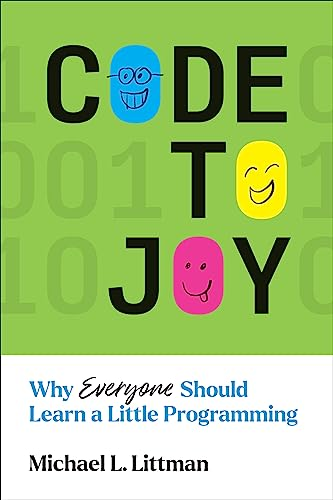
\includegraphics{Images/CodeToJoy}

\paragraph{}\textbf{Code to Joy: Why Everyone Should Learn a Little Programming} by Michael Littman. MIT, ISBN: 978-0-262-54639-3.

\section*{Course Work}\label{sec:coursework}
\paragraph{Attendance}It is important to be present for each class, though it's up to each individual student to best manage their own time. This is your time to have regular interaction with the instructor and Teaching Fellow, to ask questions, ask for specific examples, seek clarification, etc. I cannot overstate the importance of being able to ask questions and engage in dialog to help facilitate the learning process. \textbf{The students who end up being the most successful are the ones who regularly attend \underline{and} ask questions!}

\paragraph{Software}If you're using a Windows computer, you'll need to download and install Python from \href{https://www.python.org/downloads/windows/}{python.org}. If you have a Mac, Python is already installed, but you may want to install a newer version from \href{https://www.python.org/downloads/macos/}{python.org}. In both cases, make sure to install ``IDLE''. Additionally, you may wish to install PyCharm Community Edition from \url{https://www.jetbrains.com/pycharm/}. Both a free.

\paragraph{}A third option is to use Google Colabatory, available at \url{https://colab.research.google.com/} which doesn't require software installation.

\label{sec:cwhw}
\paragraph{Classwork \& Projects}Classwork will be submitted using Blackboard, and are due precisely one week after being assigned. For example, Classwork 1 is assigned on Wednesday, September 4\textsuperscript{th}, therefore the due date is 11:59 PM on Tuesday, September 19\textsuperscript{th}. Assignments may be completed early, but \underline{\hypertarget{sec:cwhw}{late assignments} will \textbf{not}} \underline{be accepted}\footnote{Late assignments may be accepted \textit{only} in the event of a documented extenuating circumstance.}. Projects are due two weeks after assignment. Classwork and Projects indicate the assignment \& due dates.

\paragraph{Quizzes}There are four quizzes and they will be held during the first 40 minutes of the class in which they're administered. The best ways to study for the quiz is to attend class, ask questions, and complete the assignments. Each quiz will focus on the materials since the quiz prior, including assigned readings, and will be \textit{cumulative}. Quizzes will be administered using the Respondus Lockdown Browser in Blackboard, so please read the following section for details on how to set it up and use it. There will be a practice quiz early in the semester to ensure everyone can use the system to ensure no surprises on quiz days.

\paragraph{LockDown Browser}This course uses the LockDown Browser for the quizzes and final exam. Watch this short video to get a basic understanding of LockDown Browser \url{http://www.respondus.com/products/lockdown-browser/student-movie.shtml}. Then download and install LockDown Browser from this link: \url{http://www.respondus.com/lockdown/download.php?id=978442813}. NOTE: This link is unique for UMBC. It cannot be used by non-UMBC students or websites outside of our campus. To take an online test, start LockDown Browser and navigate to the exam. You won't be able to access the exam with a standard web browser. For additional details on using LockDown Browser, review this FAQ \url{https://wiki.umbc.edu/x/BQb9Aw} or the Respondus Student Quick Start Guide (PDF) \url{http://respondus.com/products/lockdown-browser/guides.shtml#student}. Finally, when taking an online exam, follow these guidelines:
\begin{itemize}
\item Before starting the test, know how much time is available for it, and that you've allotted sufficient time to complete it;
\item Turn off all mobile devices, phones, etc. and don't have them within reach;
\item Remain at your desk or workstation for the duration of the quiz or exam;
\item LockDown Browser will prevent you from accessing other websites or applications; you will be unable to exit the test until all questions are completed and submitted.
\end{itemize}

\paragraph{Exams}There will be one exam, the final, which will also use the LockDown Browser. It is designed to reinforce the topics discussed throughout the semester in order to promote retention of the information.

\section*{Course Policies}
\subsection*{Grading}

\begin{center}
\begin{tabular}{ c c || c c}
\multicolumn{2}{c||}{\underline{Scale}} & \underline{Course Work} & \underline{Grade Distribution} \\
90\% - 100\% & A & Classwork & 15\% \\
80\% - 89\%  & B & Projects & 25\% \\
70\% - 79\%  & C & Quizzes & 30\% \\ 
60\% - 69\%  & D & Final Exam & 30\% \\
$<$60\%      & F & 
\end{tabular}
\end{center}

\paragraph{}For borderline grades, there may be adjustments in the student's favor based on attendance, but under no circumstances will the letter grades be lower than in the standard formula. Grades will not be ``curved'' in the sense that the percentages of A's, B's and C's are not fixed. As a guideline, a student receiving an ``A'' should be able to produce correct programs for the all of the assignments and quizzes with ease. As stated in the \hyperlink{sec:cwhw}{Classwork \& Projects} section, late work will not be accepted.

\subsection*{Academic Integrity}
\paragraph{}By enrolling is this course, each student assumes the responsibilities of an active participant in UMBC's scholarly community in which everyone's academic work and behavior are held to the highest standards of honesty. Cheating, fabrication, plagiarism, and helping others to commit these acts are all forms of academic dishonesty, and they are wrong. Academic misconduct could result in disciplinary action that may include, but is not limited to, suspension or dismissal. To find useful information about avoiding plagiarism infractions through appropriate citations, or to read the full policy regarding student academic misconduct for the graduate school, please see \url{http://www.umbc.edu/provost/integrity}.

\paragraph{}You are allowed \& \textit{encouraged} to discuss course materials with your peers! However, \underline{all assignments} \underline{are an individual effort!} Assignments will be checked for evidence of shared or copied code. If you have questions, or find that you are struggling, please ask questions, \underline{do not share code}\textbf{!}

\paragraph{}Please refrain from trying to find code online to help with your assignment. As stated a few times, if you are having trouble, then please ask for help during class, after class, or in an email. If you find yourself too tempted and do this anyway, include that URL in the assignment itself:
\begin{itemize}
\item Cite your source, don't claim it as your own,
\item If you can another student happen to use the same site and don't cite, that will be interpreted as cheating and a zero will be given for the assignment
\end{itemize}

\paragraph{ChatGPT}Do not use ChatGPT for your assignments. This doesn't help you learn, and ChatGPT has been known to give incorrect responses. You learn by doing, making mistakes, figuring out how to fix the mistakes, and repeating. Being given potential incorrect answers is not learning. If you need help with the course material, please ask questions!

\section*{Schedule}\label{sec:schedule}
\textit{Note: The schedule is subject to change. However, any changes will be thoroughly discussed and well disseminated. Please read the chapter \underline{before} class starts.}

% Fall schedule
\small
\begin{tabular}{c c l l l c}
Date    & Week & ~~~~~~~~~~~~Topic & Textbook & Code to Joy & Assignment \\ \hline
W Aug 28  & 1  & Introduction, Syllabus Review & & & \hl{Quiz 0} \\ \hline
M Sept 2  & 2  & Computers and Programs & 1 & & \\
W Sept 4  & 2  & Computers and Programs & & 1 & Classwork 1 \\
M Sept 9  & 3  & Writing Simple Programs & 2 & & \\
W Sept 11 & 3  & Writing Simple Programs & & 2, 5 & Classwork 2 \\
M Sept 16 & 4  & Computing with Numbers & 3 & & Project 1\\
W Sept 18 & 4  & Computing with Numbers & & & Classwork 3 \\
M Sept 23 & 5  & Objects and Graphics & 4 & & \\
W Sept 25 & 5  & \hl{Quiz 1} & & & \\
M Sept 30 & 6  & Sequences & 5 & & \\ \hline
W Oct 2   & 6  & Sequences & & 3 & Classwork 4 \\
M Oct 7   & 7  & Defining Functions & 6 & & Project 2\\
W Oct 9   & 7  & Defining Functions & & 7 & Classwork 5 \\
M Oct 14  & 8  & Decision Structures & 7 & & \\
W Oct 16  & 8  & \hl{Quiz 2} & & 4 & \\
M Oct 21  & 9  & Loops \& Booleans & 8 & & \\
W Oct 23  & 9  & Loops \& Booleans & & 6 & Classwork 6 \\
M Oct 28  & 10 & Simulation \& Design & 9 & & \\
W Oct 30  & 10 & Simulation \& Design & & & Classwork 7 \\ \hline
M Nov 4   & 11 & Defining Classes & 10 & & Project 3\\
W Nov 6   & 11 & \hl{Quiz 3} & & & \\
M Nov 11  & 12 & Defining Classes & & & \\
W Nov 13  & 12 & Data Collections & 11 & &  \\
M Nov 18  & 13 & Data Collections & & 8 & Classwork 8\\
W Nov 20  & 13 & Object Oriented Design & 12 & & \\
M Nov 25  & 14 & Object Oriented Design & & & Classwork 9 \\
W Nov 27  & 14 & \hl{Quiz 4} & & & \\ \hline
M Dec 2   & 15 & Algorithm Design \& Recursion & 13 & & \\
W Dec 4   & 15 & Algorithm Design \& Recursion & & 9 & Classwork 10 \\
M Dec 9   & 16 & Review & & & \\
W Dec 11  & 16 & \hl{Study Day, no class} & & & \\
M Dec 16  & 17 & \hl{Final Exam? TBD.} & & & \\
\end{tabular}

% Spring schedule goes here

\section*{Accessibility \& Disability Accommodations, Guidance \& Resources}
\paragraph{}Accommodations for students with disabilities are provided for all students with a qualified disability under the Americans with Disabilities Act (ADA \& ADAAA) and Section 504 of the Rehabilitation Act who request and are eligible for accommodations. The Office of Student Disability Services (SDS) is the UMBC department designated to coordinate accommodations that creates equal access for students when barriers to participation exist in University courses, programs, or activities.

\paragraph{}If you have a documented disability and need to request academic accommodations in your courses, please refer to the SDS website at \url{http://sds.umbc.edu} for registration information and office procedures.
\begin{itemize}
\item SDS email: \href{mailto:disAbility@umbc.edu}{disAbility@umbc.edu}
\item SDS phone: \href{tel:+14104552459}{(410) 455-2459}
\end{itemize}
If you will be using SDS approved accommodations in this class, please contact the instructor to discuss implementation of the accommodations. During remote instruction requirements due to COVID, communication and flexibility will be essential for success.

\section*{Sexual Assault, Sexual Harassment, \& Gender Based Violence \& Discrimination}
\paragraph{}UMBC Policy\footnote{\url{https://oei.umbc.edu/gender-discrimination-sexual-misconduct/}} and Federal law (Title IX) prohibit discrimination and harassment on the basis of sex, sexual orientation, and gender identity in University programs and activities. Any student who is impacted by sexual harassment, sexual assault, domestic violence, dating violence, stalking, sexual exploitation, gender discrimination, pregnancy discrimination, gender-based harassment or retaliation should contact the University’s Title IX Coordinator\footnote{\url{https://oei.umbc.edu/title-ix-coordinator/}} to make a report and/or access support and resources:
\begin{itemize}
\item Mikhel A. Kushner, Title IX Coordinator (she/they)
\item \href{tel:+14104551250}{(410) 455-1250} (direct line), \href{mailto:kushner@umbc.edu?Subject=Title\%20IX}{kushner@umbc.edu}
\end{itemize}

\paragraph{}You can access support and resources even if you do not want to take any further action. You will not be forced to file a formal complaint or police report. Please be aware that the University may take action on its own if essential to protect the safety of the community. If you are interested in or thinking about making a report, please use the Online Reporting/Referral Form. Please note that, if you report anonymously,  the University’s ability to respond will be limited.

\section*{Resources to Help you Succeed}
\paragraph{}Click on the following links for helpful resources:
UMBC’s Academic Success Center (ASC) \url{https://academicsuccess.umbc.edu/} provides a range of resources to support students as they progress toward degree completion. They will continue to offer all of their services online. 
The ASC has created a specialized set of Online Learning Resources \url{https://lrc.umbc.edu/online_learning/}, including videos and guides to help students succeed while learning online.
In addition, check out the following resources:

\begin{itemize}
\item Academic Success Center Resources \url{https://academicsuccess.umbc.edu/asc-business-continuity/} include: Online tutoring and writing support, supplemental instruction/peer-assisted study sessions (SI PASS), placement testing, FYI academic alerts, success courses, academic advocacy, academic policy and academic success meetings.

\item Tutoring and Writing Center Appointments \url{https://lrc.umbc.edu/tutor/}b will be online; students can make appointments by going to \url{https://saml2.go-redrock.com/relay.php}.

\item SI PASS \url{https://si.lrc.umbc.edu/} Supplemental Instruction (SI)/ Peer Assisted Study Sessions (PASS). The SI PASS program targets traditionally difficult academic courses, providing regularly scheduled, out-of-class review sessions, happening in Blackboard Collaborate inside your existing Blackboard course.

\item Academic Advocates: Advocates work one-on-one with students who need support navigating academic and institutional challenges, no matter how complex the concerns (i.e., personal, academic, or financial). \url{https://academicadvocacy.umbc.edu/student-referrals/submit-a-referral/}

\item Academic Success Meetings - Schedule a one-to-one virtual meeting with an Academic Success Center Professional who can help you with time management, study skills, and accessing campus resources. \url{https://lrc.umbc.edu/academic-success-meeting/}

\end{itemize}

If you have a question, please contact the ASC at \href{mailto:academicsuccess@umbc.edu}{academicsuccess@umbc.edu}.
\end{document}
